% =============================================================================
% chap_03.tex  —  Emulation and Simulation Framework
% =============================================================================

\chapter{Emulation and Simulation Framework}
\label{chap:emulation}

\section*{Introduction}
Before deploying inference workloads on the physical NXP i.MX~8M~Plus board,
it is essential to establish a reproducible performance baseline and to develop
a realistic estimation of what the target hardware can deliver. This chapter
presents a three-methodology framework that progressively builds from a
measured x86~CPU baseline, through a physics-based simulation of the ARM
Cortex-A53 CPU and Vivante GC7000UltraLite NPU, to an attempted QEMU
user-mode ARM64 emulation. Together, these methodologies provide a
comprehensive pre-hardware characterisation of the six ONNX models introduced
in Chapter~2, enabling informed decisions about model selection and deployment
strategy before physical access to the target platform is available.

The chapter is organised as follows.
Section~\ref{sec:pipeline_overview} presents the shared pipeline infrastructure
common to all three methodologies.
Section~\ref{sec:m1_design} details Methodology~1, the x86~CPU baseline.
Section~\ref{sec:m2_design} describes Methodology~2, the physics-based
tri-path simulation.
Section~\ref{sec:m3_design} documents Methodology~3, the QEMU emulation
attempt and the reasons for its abandonment.
Section~\ref{sec:architectural_design} presents the architectural design of
the emulation environment.
Section~\ref{sec:technology_choices} justifies the key technology choices and
simulation parameters.
Finally, Section~\ref{sec:m_results} summarises the comparative results across
methodologies.

% =============================================================================
\section{Shared Pipeline Infrastructure}
\label{sec:pipeline_overview}
% =============================================================================

All three methodologies share a common four-stage pipeline skeleton that
ensures consistency in model handling, data flow, and metric computation.

\subsection{Four-Stage Pipeline Structure}

Every benchmarking run, regardless of methodology, follows the same four-stage
structure:

\begin{enumerate}[leftmargin=2em, itemsep=1pt, topsep=3pt]
    \item \textbf{Setup:} Model export to ONNX opset~17 with weight integrity
          verification, and dataset construction from Tiny-ImageNet-200.
    \item \textbf{Inference:} A pipelined producer--consumer architecture
          where preprocessing and inference are decoupled, with isolated
          inference timing.
    \item \textbf{Metrics:} Statistical computation of latency distributions
          (mean, median, p95, p99, standard deviation, IQR, coefficient of
          variation), throughput, and top-1 accuracy for classification models.
    \item \textbf{Visualisation:} Generation of latency-over-time traces,
          histogram/KDE distributions, comparative bar charts, and
          accuracy--latency Pareto scatter plots.
\end{enumerate}

\begin{figure}[H]
\centering
\begin{tikzpicture}[
    box/.style={rectangle, rounded corners=4pt, draw=accent, fill=codebg,
                minimum width=2.8cm, minimum height=0.9cm,
                text centered, font=\small\bfseries},
    arr/.style={->, thick, color=accent},
    note/.style={font=\footnotesize\itshape, color=codegray}
]
    \node[box] (setup) at (0,0)    {Setup};
    \node[box] (inf)   at (3.5,0)  {Inference};
    \node[box] (met)   at (7,0)    {Metrics};
    \node[box] (viz)   at (10.5,0) {Visualise};
    \draw[arr] (setup) -- (inf);
    \draw[arr] (inf)   -- (met);
    \draw[arr] (met)   -- (viz);
    \node[note] at (0,-1.1)    {ONNX opset 17};
    \node[note] at (3.5,-1.1)  {producer--consumer};
    \node[note] at (7,-1.1)    {throughput / accuracy};
    \node[note] at (10.5,-1.1) {PNG plots};
\end{tikzpicture}
\caption{Shared four-stage pipeline common to all three methodologies.}
\label{fig:pipeline_overview}
\end{figure}

\subsection{Model Zoo}

Six ONNX models are evaluated across all methodologies.
Table~\ref{tab:model_zoo} summarises their characteristics.

\begin{table}[H]
\centering
\caption{Model registry and characterisation.}
\label{tab:model_zoo}
\begin{tabular}{lcccccc}
\toprule
\textbf{Model} & \textbf{Input} & \textbf{Classes} & \textbf{Task}
    & \textbf{Source} & \textbf{Min~MB} & \textbf{Top-1} \\
\midrule
ResNet50-v1.5       & $224^2$ & 1000 & cls & torchvision & 90  & $\approx76\%$ \\
MobileNetV2         & $224^2$ & 1000 & cls & torchvision & 12  & $\approx72\%$ \\
MobileNetV3-Small   & $224^2$ & 1000 & cls & torchvision &  8  & $\approx67\%$ \\
MobileNetV1-1.0     & $224^2$ & 1000 & cls & timm        & 14  & $\approx71\%$ \\
EfficientNet-Lite0  & $224^2$ & 1000 & cls & timm        & 15  & $\approx74\%$ \\
SSD-MBv2-backbone   & $300^2$ &  --- & det & torchvision & 10  & N/A \\
\bottomrule
\end{tabular}
\end{table}

\noindent\textbf{timm dependency.}\quad Only \texttt{MobileNetV1} and
\texttt{EfficientNet-Lite0} require the \texttt{timm} library
(\texttt{pip install timm}). All other models depend only on \texttt{torch},
\texttt{torchvision}, \texttt{onnxruntime}, \texttt{numpy}, and
\texttt{pillow}.

\subsection{Dataset Construction}

\subsubsection{Tiny-ImageNet-200 Validation Set}

Tiny-ImageNet-200 is a 200-class subset of ImageNet distributed by Stanford
CS231n~\cite{ref:tiny-imagenet}. The validation partition contains 10\,000
JPEG images ($64\times64$ pixels, 50 per class), annotated with WordNet~IDs
(WNIDs). A handcrafted lookup table $\phi$ maps each WNID to its canonical
ImageNet-1k class index (0--999):
\begin{equation}
    \phi : \text{WNID} \rightarrow \{0, \ldots, 999\} \subset \mathbb{Z}
    \label{eq:wnid}
\end{equation}
All 10\,000 validation images are selected with a fixed random seed
(\texttt{seed=42}). The archive ($\approx$236~MB) is cached locally so that
subsequent runs skip the download.

\subsubsection{Preprocessing Pipeline}
\label{sec:preproc_pipeline}

The models were pre-trained on full ImageNet at $224\times224$ pixels. Since
Tiny-ImageNet images are natively $64\times64$, a three-step preprocessing
pipeline is applied identically across all inference paths:

\begin{figure}[H]
\centering
\begin{tikzpicture}[
    box/.style={rectangle, rounded corners=4pt, draw=accent, fill=codebg,
                minimum width=2.6cm, minimum height=0.9cm,
                text centered, font=\small\bfseries},
    arr/.style={->, thick, color=accent},
    note/.style={font=\footnotesize\itshape, color=codegray}
]
    \node[box] (inp)  at (0,0)    {Input};
    \node[box] (res)  at (3.2,0)  {Resize};
    \node[box] (crp)  at (6.4,0)  {Crop};
    \node[box] (nrm)  at (9.6,0)  {Normalise};
    \node[box] (out)  at (12.8,0) {Output};
    \draw[arr] (inp) -- (res);
    \draw[arr] (res) -- (crp);
    \draw[arr] (crp) -- (nrm);
    \draw[arr] (nrm) -- (out);
    \node[note] at (0,-1.1)    {$64\times64$ RGB};
    \node[note] at (3.2,-1.1)  {$64\to256$~px};
    \node[note] at (6.4,-1.1)  {$224\times224$};
    \node[note] at (9.6,-1.1)  {$\mu,\sigma$ ImageNet};
    \node[note] at (12.8,-1.1) {$1\times3\times224\times224$};
\end{tikzpicture}
\caption{Tiny-ImageNet preprocessing pipeline applied identically on every
inference path.}
\label{fig:preproc_pipeline}
\end{figure}

\begin{enumerate}[itemsep=1pt, topsep=3pt]
    \item \textbf{Bilinear resize:} The image is resized so that its shorter
          dimension equals 256~px, preserving aspect ratio. PIL
          \texttt{BILINEAR} interpolation is used, consistent with the
          standard ImageNet evaluation protocol.

    \item \textbf{Centre crop to $224\times224$:} A $224\times224$ region is
          extracted from the centre of the $256\times256$ intermediate. The
          crop offsets are:
          \begin{equation}
              \text{left} = \lfloor(W-224)/2\rfloor,\quad
              \text{top}  = \lfloor(H-224)/2\rfloor
          \end{equation}
          where $W$ and $H$ are the width and height of the resized image.

    \item \textbf{Normalisation:} Each pixel value is scaled to $[0,1]$ by
          dividing by 255, then standardised channel-wise:
          \begin{equation}
              x_c^{\prime} = \frac{x_c/255 - \mu_c}{\sigma_c},\quad
              c\in\{R,G,B\},\quad
              \mu=[0.485,0.456,0.406],\quad
              \sigma=[0.229,0.224,0.225]
          \end{equation}
\end{enumerate}

The output is a \texttt{float32} NumPy array of shape $[1,3,224,224]$,
memory footprint $\approx0.60$~MB. This tensor's DMA transfer from LPDDR4
into NPU SRAM constitutes the fixed overhead $\Delta_{\text{DMA}}=0.18$~ms
in the NPU simulation (Section~\ref{sec:m2_npu_sim}).

\paragraph{Impact on accuracy.}
Upsampling from $64\times64$ to $224\times224$ introduces bilinear blur not
present during training. Top-1 accuracy is consequently 16\%--31\% versus the
69\%--80\% these models achieve on genuine ImageNet data. Accuracy is treated
as a \emph{sanity check}: values well above the $\approx0.1\%$ random
baseline confirm correct model loading, label remapping, and preprocessing
integrity. Latency measurements — the primary benchmark output — are
unaffected by the resolution mismatch.

% =============================================================================
\section{Methodology 1: x86 CPU Baseline}
\label{sec:m1_design}
% =============================================================================

\subsection{Overview}

Methodology~1 establishes a reproducible performance baseline by executing
unmodified \texttt{float32} ONNX models on an AMD Ryzen~5 5600H using ONNX
Runtime's \texttt{CPUExecutionProvider}. This serves two purposes: (1)
confirming that pretrained weights are correctly loaded and characterising
accuracy under the Tiny-ImageNet resolution mismatch, and (2) providing
reference latency measurements for relative comparison with the
simulation-based methodologies.

\subsection{ONNX Runtime Session Configuration}

Sessions are created with full graph optimisation enabled. The number of
intra-op and inter-op threads is set to~0 (auto), allowing ONNX Runtime to
utilise all available physical cores for maximum parallelism.

\begin{lstlisting}[language=Python,
    caption={ONNX Runtime session creation with full graph optimisation.}]
opts = ort.SessionOptions()
opts.intra_op_num_threads     = 0   # auto = all physical cores
opts.inter_op_num_threads     = 0
opts.graph_optimization_level = ort.GraphOptimizationLevel.ORT_ENABLE_ALL
opts.enable_profiling         = False

session = ort.InferenceSession(
    model_path,
    sess_options=opts,
    providers=["CPUExecutionProvider"]
)
\end{lstlisting}

\subsection{Producer--Consumer Pipeline}

To prevent preprocessing from inflating inference timing, a
producer--consumer architecture decouples JPEG decode/resize from ONNX
session execution:

\begin{itemize}[itemsep=1pt, topsep=3pt]
    \item \textbf{Producer:} A \texttt{ThreadPoolExecutor} with 4 workers
          preprocesses images and submits ready tensors to a bounded queue
          (capacity 32). The producer maintains the original image index,
          preserving the link between image, tensor, and ground-truth label.
    \item \textbf{Consumer:} The main thread pulls pre-built tensors from the
          queue and calls \texttt{session.run()} sequentially, recording
          per-inference latency.
\end{itemize}

\begin{figure}[H]
\centering
\begin{tikzpicture}[
    box/.style={rectangle, rounded corners=4pt, draw=accent, fill=codebg,
                minimum width=3.0cm, minimum height=0.9cm,
                text centered, font=\small\bfseries},
    arr/.style={->, thick, color=accent}
]
    \node[box] (disk)  at (0,0)   {Disk};
    \node[box] (pool)  at (3.5,0) {ThreadPool};
    \node[box] (queue) at (7,0)   {Tensor Queue};
    \node[box] (ort)   at (10.5,0){ONNX Runtime};
    \node[box] (out)   at (10.5,-2){Results Buffer};
    \draw[arr] (disk)  -- (pool);
    \draw[arr] (pool)  -- (queue);
    \draw[arr] (queue) -- (ort);
    \draw[arr] (ort)   -- (out);
\end{tikzpicture}
\caption{Producer--consumer inference pipeline for Methodology~1.}
\label{fig:m1_pipeline}
\end{figure}

\subsection{Timing Isolation}

Only the \texttt{session.run()} call is timed using
\texttt{time.perf\_counter()}:
\begin{equation}
    t_{\text{inf},i} = t_1 - t_0,\quad
    t_0 = \texttt{perf\_counter()\ before},\quad
    t_1 = \texttt{perf\_counter()\ after}
\end{equation}
Preprocessing time is recorded separately as an overlapped cost and does not
contribute to the inference latency histogram.

\subsection{Warm-up Protocol}

Five initial inference calls are executed before timing begins and excluded
from all latency statistics. This protocol: (1) completes ONNX Runtime JIT
compilation, (2) warms CPU instruction caches and the TLB, and (3) initialises
BLAS thread pools and numerical libraries.

\subsection{Inference Algorithm}

\begin{algorithm}[H]
\caption{Methodology~1 Baseline Inference Benchmark}
\label{alg:m1_inference}
\begin{algorithmic}[1]
\Require Model $\mathcal{M}$, dataset $\mathcal{D}=\{(x_i,y_i)\}_{i=0}^{N-1}$,
         $W=5$, $Q=16$, $P=4$
\Ensure Latency vector $\mathbf{L}\in\mathbb{R}^N$, accuracy $A$
\State Create ORT session $S$ with \texttt{ORT\_ENABLE\_ALL}
\For{$w=1\ldots W$}
    \State $S.\texttt{run}(\texttt{preprocess}(x_0))$ \Comment{warm-up, discarded}
\EndFor
\State Start producer with $P$ workers, queue capacity $2Q$
\For{$i=0\ldots N-1$}
    \State $(i',\hat{x},t_\text{pp})\gets\mathcal{Q}.\texttt{get}()$
    \State $t_0\gets\texttt{perf\_counter}()$
    \State $\hat{y}\gets S.\texttt{run}(\hat{x})$
    \State $t_1\gets\texttt{perf\_counter}()$
    \State $L_{i'}\gets(t_1-t_0)\times1000$ \Comment{ms}
    \If{task $=$ \texttt{cls}}
        \State $\text{correct}_{i'}\gets\mathbf{1}[\arg\max\hat{y}=y_{i'}]$
    \EndIf
\EndFor
\State $A\gets\frac{1}{N}\sum\text{correct}_i\times100$ \textbf{if} cls \textbf{else} \textsc{None}
\State \Return $\mathbf{L}$, $A$
\end{algorithmic}
\end{algorithm}

\subsection{Statistical Metrics}

For each model, the latency vector $\mathbf{L}=(L_0,\ldots,L_{N-1})$ in
milliseconds yields:

\begin{itemize}[itemsep=1pt, topsep=3pt]
    \item \textbf{Mean:} $\bar{L}=\frac{1}{N}\sum L_i$
    \item \textbf{Median (p50):} $L_{0.50}$, the typical latency
    \item \textbf{p95:} $L_{0.95}$, the SLA tail
    \item \textbf{p99:} $L_{0.99}$, the strict tail used in MLPerf
    \item \textbf{Std:} $\sigma=\sqrt{\frac{1}{N}\sum(L_i-\bar{L})^2}$
    \item \textbf{IQR:} $L_{0.75}-L_{0.25}$
    \item \textbf{Throughput:} $T=1000/\bar{L}$ img/s
    \item \textbf{CV:} $\sigma/\bar{L}$; $<0.10$ stable, $\in[0.10,0.30)$
          moderate jitter, $\geq0.30$ high jitter
\end{itemize}

\subsection{Experimental Setup}

\begin{table}[H]
\centering
\caption{Host hardware and software environment for Methodology~1.}
\label{tab:m1_env}
\begin{tabular}{ll}
\toprule
\textbf{Parameter} & \textbf{Value} \\
\midrule
Hardware             & x86-64 AMD Ryzen~5 5600H \\
Runtime              & ONNX Runtime \texttt{CPUExecutionProvider} \\
Batch size           & 1 (sequential) \\
Warm-up runs         & 5 (excluded from timing) \\
Preprocessing workers& 4 threads (\texttt{ThreadPoolExecutor}) \\
Queue depth          & 32 tensors \\
Dataset              & Tiny-ImageNet-200 validation, $N=10{,}000$ \\
Label space          & ImageNet-1k (0--999) \\
\bottomrule
\end{tabular}
\end{table}

\subsection{Results}

\subsubsection{Latency and Throughput}

\begin{table}[H]
\centering
\caption{Latency and throughput results --- x86 CPU baseline.}
\label{tab:m1_results_lat}
\resizebox{\textwidth}{!}{%
\begin{tabular}{lcccccccc}
\toprule
\textbf{Model} & \textbf{Task} & \textbf{$\bar{L}$ (ms)} & \textbf{p50}
    & \textbf{p95} & \textbf{p99} & \textbf{$\sigma$} & \textbf{CV}
    & \textbf{img/s} \\
\midrule
ResNet50-v1.5       & cls & 22.74 & 19.24 & 41.37 & 66.39 & 9.52 & 0.419 & 43.98 \\
MobileNetV2         & cls &  4.58 &  4.15 &  7.68 & 11.82 & 1.96 & 0.429 & 218.52 \\
MobileNetV3-Small   & cls &  3.45 &  3.43 &  5.32 &  7.35 & 1.20 & 0.348 & 289.89 \\
MobileNetV1-1.0     & cls &  6.05 &  5.20 & 11.06 & 17.89 & 2.80 & 0.464 & 165.39 \\
EfficientNet-Lite0  & cls &  5.45 &  4.85 &  9.31 & 14.37 & 2.39 & 0.438 & 183.43 \\
SSD-MBv2-backbone   & det &  7.87 &  6.81 & 13.51 & 24.72 & 3.69 & 0.469 & 127.01 \\
\bottomrule
\end{tabular}}
\end{table}

\subsubsection{Visualisation Suite}

\paragraph{Latency over time.}
Per-image latency trace overlaid with mean $\bar{L}$, p95, and $\pm1\sigma$
band. A flat trace indicates thermal and frequency stability; a rising trend
indicates thermal throttling; spikes indicate OS scheduling jitter.

\subsection{Latency Distribution: Histogram and KDE Visualisation}

Combined histogram and Gaussian KDE with Scott's bandwidth rule
$h = n^{-1/5}\cdot\sigma$. Mean and p95 are marked with dashed/dotted
vertical lines. A narrow tall peak indicates consistent performance; a heavy
right tail signals occasional stalls.

\begin{figure}[H]
    \centering
    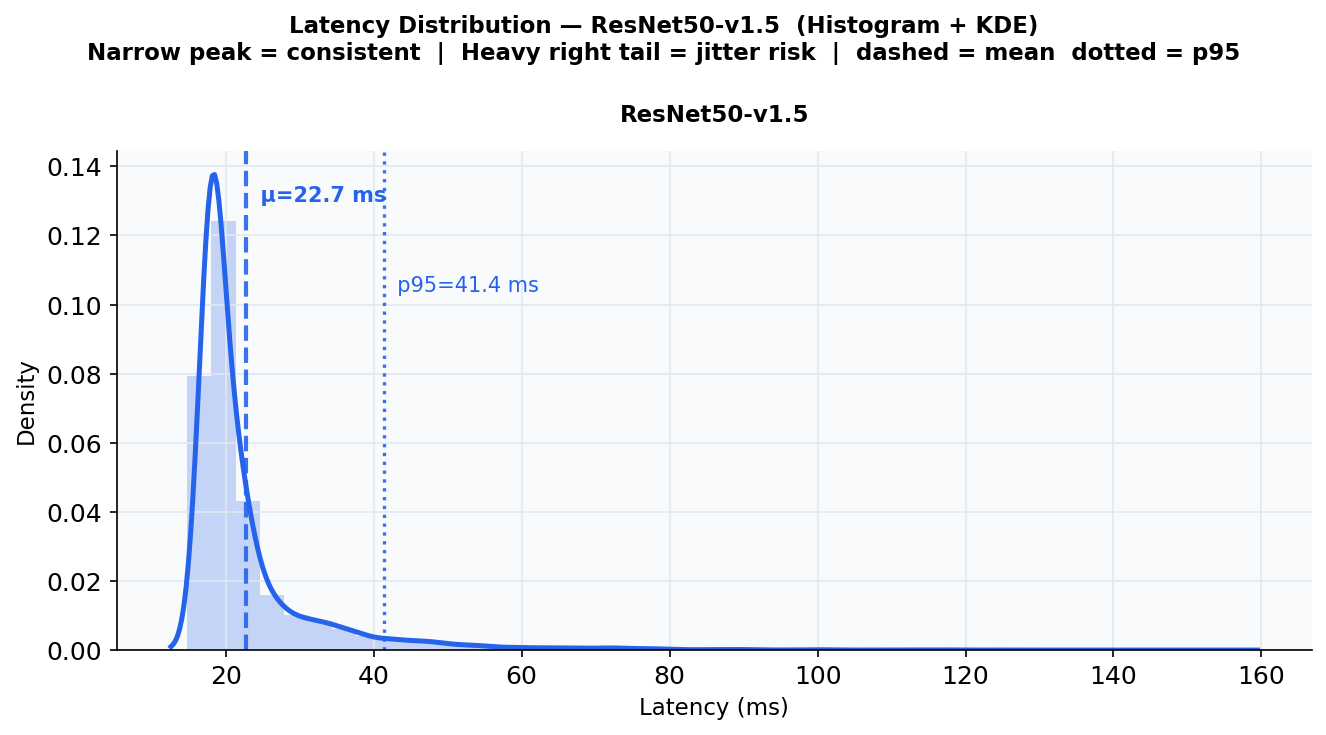
\includegraphics[width=\textwidth]{img/pics updated hiararchy pfe/Latency Distribution/1-242-1.png}
    \caption{Latency distribution --- ResNet50-v1.5.}
    \label{fig:m1_hist_resnet50}
\end{figure}

\begin{figure}[H]
    \centering
    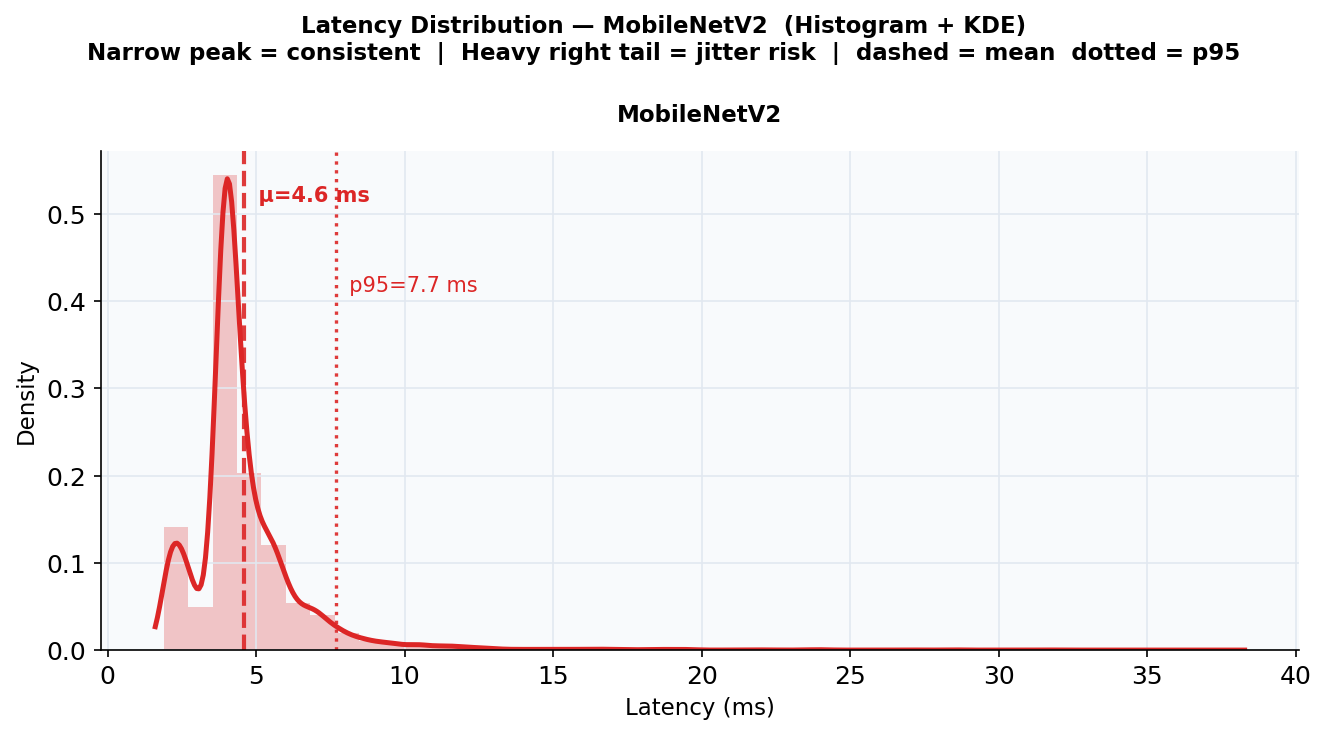
\includegraphics[width=\textwidth]{img/pics updated hiararchy pfe/Latency Distribution/1-242-2.png}
    \caption{Latency distribution --- MobileNetV2.}
    \label{fig:m1_hist_mbv2}
\end{figure}

\begin{figure}[H]
    \centering
    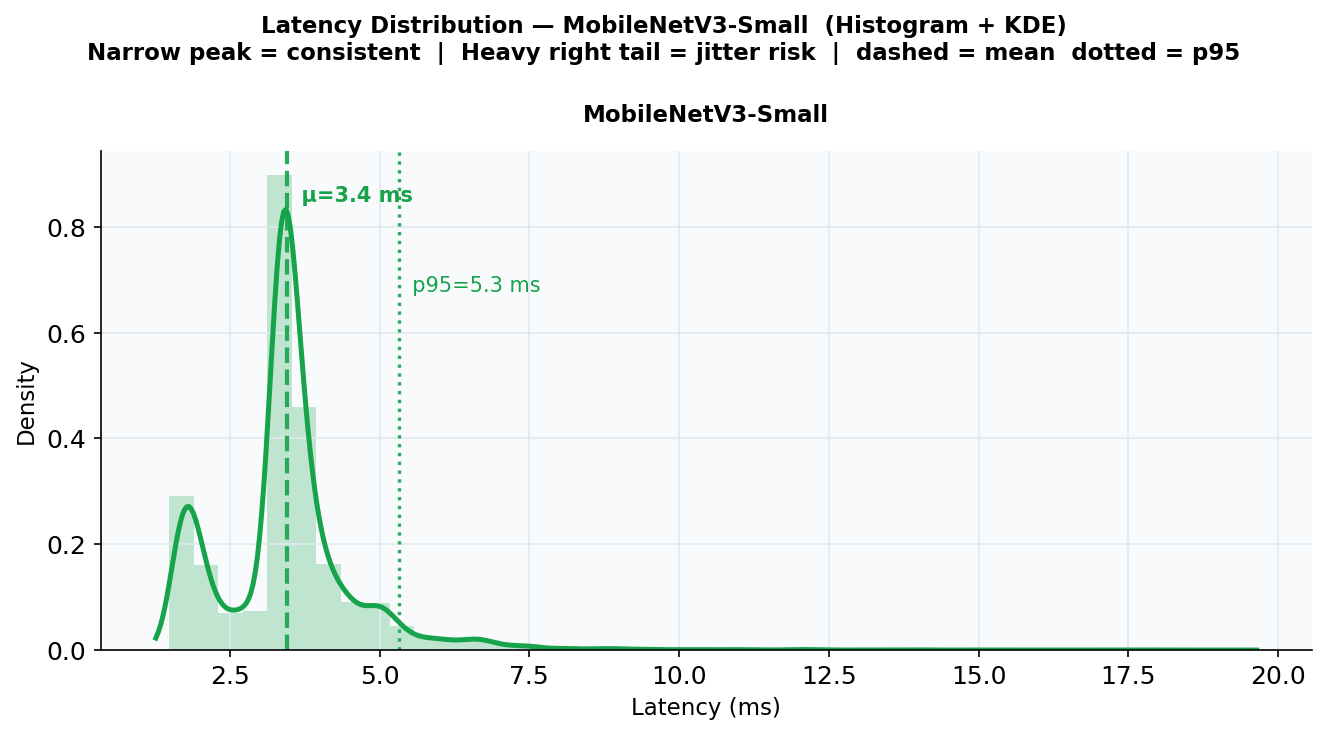
\includegraphics[width=\textwidth]{img/pics updated hiararchy pfe/Latency Distribution/1-242-3.png}
    \caption{Latency distribution --- MobileNetV3-Small.}
    \label{fig:m1_hist_mbv3small}
\end{figure}

\begin{figure}[H]
    \centering
    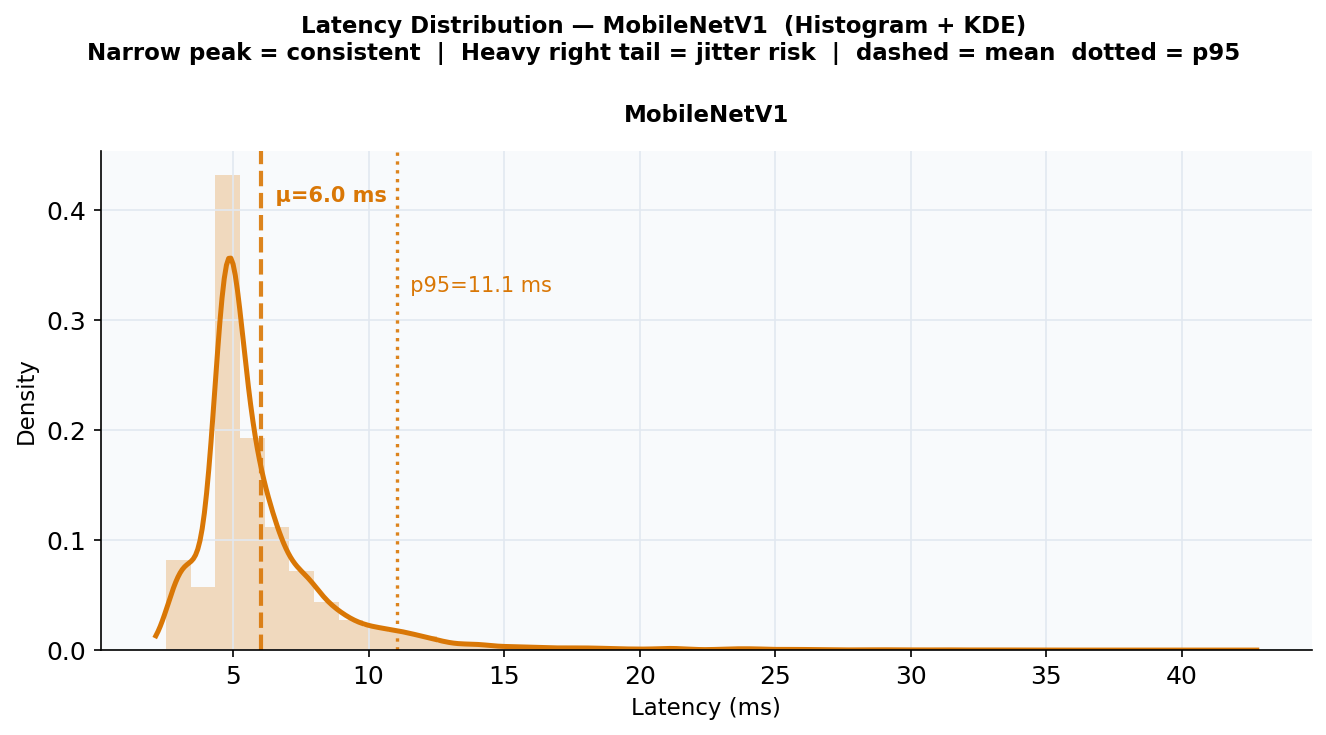
\includegraphics[width=\textwidth]{img/pics updated hiararchy pfe/Latency Distribution/1-242-4.png}
    \caption{Latency distribution --- MobileNetV1.}
    \label{fig:m1_hist_mbv1}
\end{figure}

\begin{figure}[H]
    \centering
    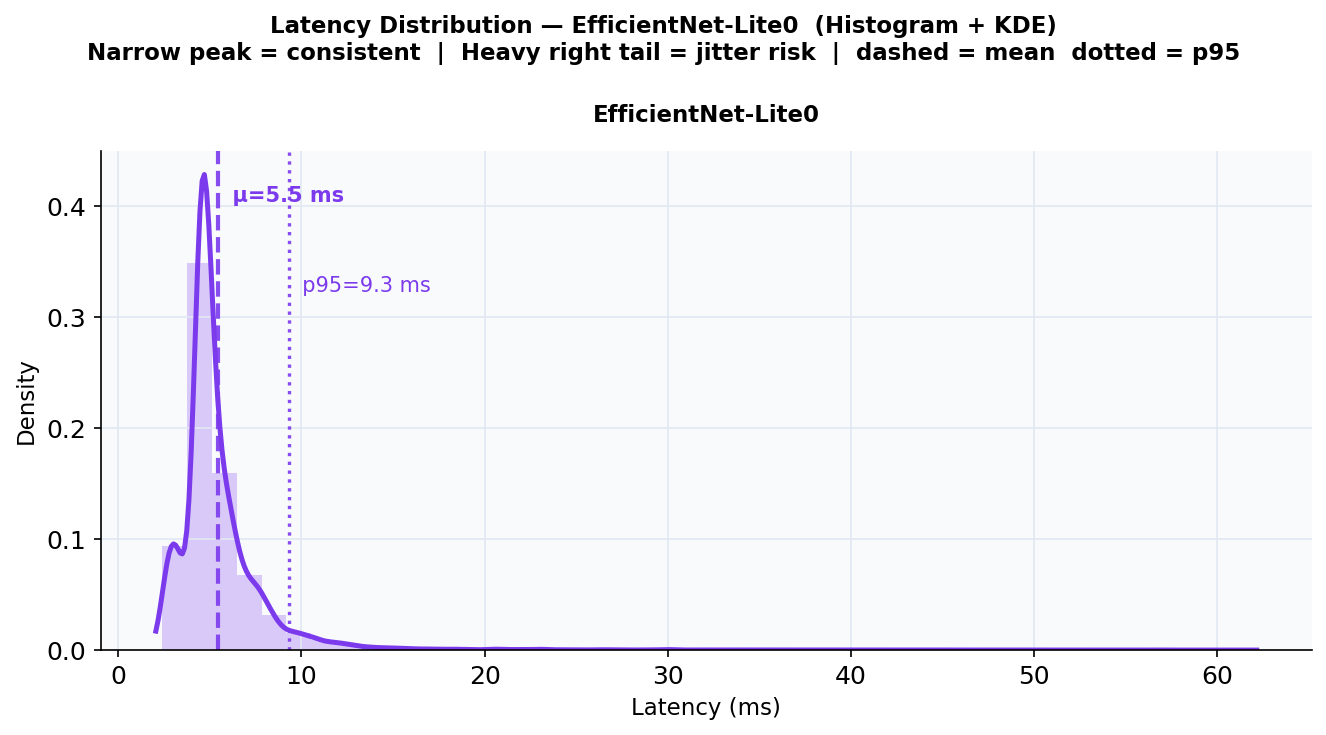
\includegraphics[width=\textwidth]{img/pics updated hiararchy pfe/Latency Distribution/1-242-5.png}
    \caption{Latency distribution --- EfficientNet-Lite0.}
    \label{fig:m1_hist_effnet}
\end{figure}

\begin{figure}[H]
    \centering
    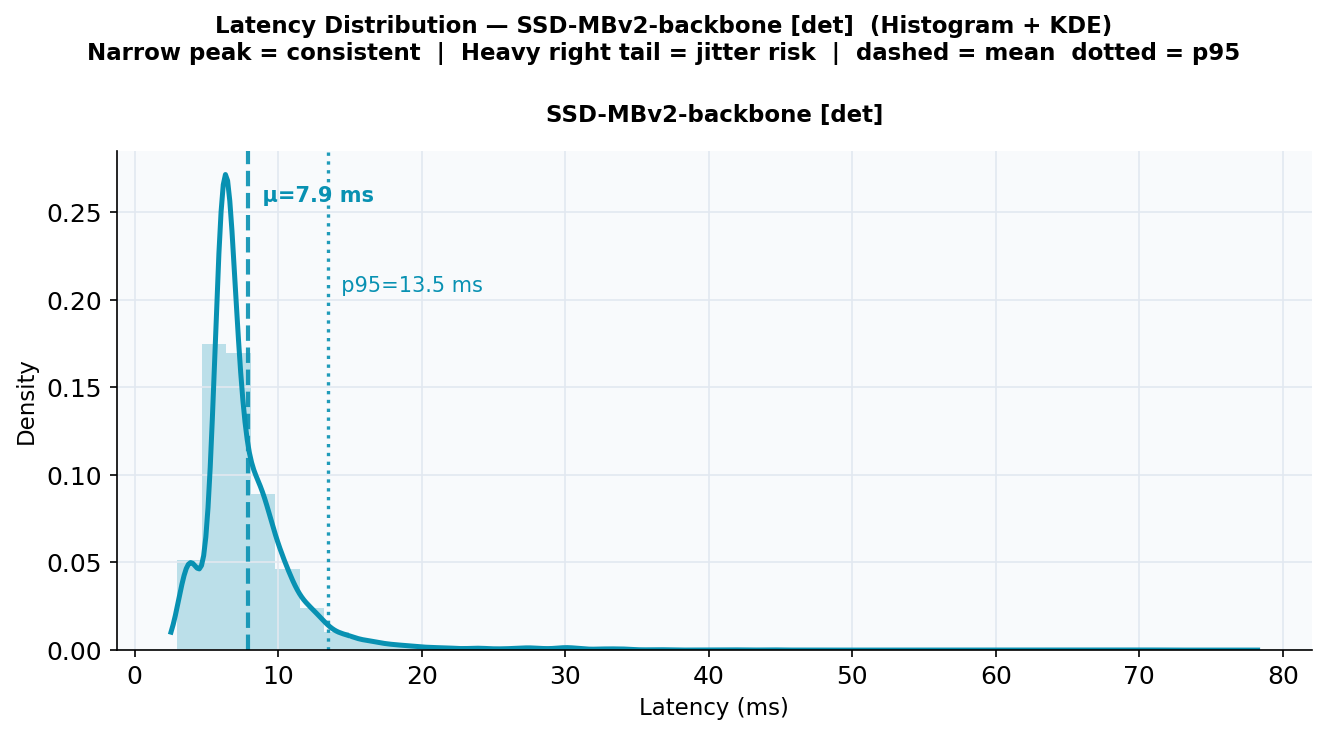
\includegraphics[width=\textwidth]{img/pics updated hiararchy pfe/Latency Distribution/1-242-6.png}
    \caption{Latency distribution --- SSD-MBv2-backbone.}
    \label{fig:m1_hist_ssd}
\end{figure}
\paragraph{Latency distribution (histogram + KDE).}
Combined histogram and Gaussian KDE with Scott's bandwidth rule
$h=n^{-1/5}\cdot\sigma$. Mean and p95 are marked with dashed/dotted vertical
lines. A narrow tall peak indicates consistent performance; a heavy right tail
signals occasional stalls.

% ---- PLACEHOLDER: Histogram+KDE plots (Methodology 1) ----
% \begin{figure}[H]
%     \centering
%     \includegraphics[width=\textwidth]{vis/m1_hist_resnet50.png}
%     \caption{Latency distribution --- ResNet50-v1.5.}
%     \label{fig:m1_hist_resnet}
% \end{figure}
% ... (repeat for the remaining five models)

\paragraph{Preprocessing vs.\ inference time breakdown.}

% ---- PLACEHOLDER: Time breakdown stacked bar (Methodology 1) ----
% \begin{figure}[H]
%     \centering
%     \includegraphics[width=\textwidth]{vis/m1_time_breakdown.png}
%     \caption{Preprocessing vs.\ inference time breakdown (x86 CPU baseline).}
%     \label{fig:m1_breakdown}
% \end{figure}

\paragraph{Accuracy--latency Pareto scatter.}
The Pareto frontier connects all models not dominated by any other candidate.
A model is dominated if there exists another with simultaneously higher
accuracy \emph{and} lower latency. Accuracy figures are indicative
(Tiny-ImageNet upsampling degrades all models uniformly), but relative
positions and the frontier are valid for comparative analysis.

% ---- PLACEHOLDER: Pareto scatter (Methodology 1) ----
% \begin{figure}[H]
%     \centering
%     \includegraphics[width=\textwidth]{vis/m1_pareto.png}
%     \caption{Accuracy--latency Pareto scatter for classification models
%              (x86 CPU baseline).}
%     \label{fig:m1_pareto}
% \end{figure}

% =============================================================================
\section{Methodology 2: Physics-Based ARM and NPU Simulation}
\label{sec:m2_design}
% =============================================================================

\subsection{Overview and Motivation}

Methodology~2 extends the x86 baseline by simulating what inference would look
like on the NXP i.MX~8M~Plus embedded board before physical hardware is
available. The simulation executes entirely on the host x86 machine and
produces three latency estimates for every inference call — a \emph{tri-path}
execution:

\begin{description}[itemsep=1pt, topsep=3pt]
    \item[\textbf{Path~A — x86 Host (measured):}] The actual wall-clock time
          of a real ONNX Runtime forward pass on the host CPU.
    \item[\textbf{Path~B — ARM Cortex-A53 CPU (simulated):}] An estimate of
          how long the same model would take on the ARM Cortex-A53 processor,
          derived by applying a sequence of six physical effects to the real
          x86 measurement.
    \item[\textbf{Path~C — Vivante GC7000UltraLite NPU (simulated):}] An
          estimate of NPU inference latency, anchored to a calibration mean
          and independent of per-image x86 measurements.
\end{description}

Accuracy is identical across all three paths because the logits come from a
single real ONNX Runtime forward pass. Only \emph{latency} differs.

\subsection{Target Hardware Specification}

\begin{table}[H]
\centering
\caption{NXP i.MX~8M~Plus hardware specification targeted by the simulation.}
\label{tab:imx8_spec}
\begin{tabular}{ll}
\toprule
\textbf{Component} & \textbf{Specification} \\
\midrule
SoC         & NXP i.MX~8M~Plus \\
CPU cluster & 4$\times$ ARM Cortex-A53 @ 1.8~GHz \\
SIMD        & ARMv8-A NEON (128-bit vector width) \\
NPU         & Vivante GC7000UltraLite, 2.3~TOPS (INT8) \\
RAM         & 4~GB LPDDR4 @ 25.6~GB/s peak \\
OS          & Yocto Linux (single-user embedded profile) \\
\bottomrule
\end{tabular}
\end{table}

\subsection{Tri-Path Architecture and Two-Pass Strategy}

A circular dependency exists: the NPU simulator needs the ARM CPU mean latency
before it can set its base, but that mean is only known after the ARM CPU
simulator has processed images. The implementation resolves this with a
two-pass approach:

\begin{enumerate}[itemsep=1pt, topsep=3pt]
    \item \textbf{Calibration pass (200 images):} Real ONNX Runtime forward
          passes yield $\bar{L}_{\text{x86}}^{\text{calib}}$. The ARM CPU
          calibration mean is:
          \begin{equation}
              \bar{L}_{\text{ARM}}^{\text{calib}}
              = \bar{L}_{\text{x86}}^{\text{calib}} \times s_{\text{cpu}}
          \end{equation}
          The NPU base latency is then fixed as:
          \begin{equation}
              L_{\text{NPU}}^{\text{base}}
              = \bar{L}_{\text{ARM}}^{\text{calib}} \times s_{\text{NPU}}
          \end{equation}

    \item \textbf{Full benchmark pass ($N$ images):} For every image, one
          real forward pass produces $L_i^{\text{x86}}$ and output logits.
          Path~B receives $L_i^{\text{x86}}$ and applies the six-effect
          physics model; Path~C takes no per-image input and estimates NPU
          latency analytically.
\end{enumerate}

\subsection{Path B: ARM Cortex-A53 CPU Simulator}
\label{sec:m2_arm_cpu_sim}

The \texttt{ARMCPUSimulator} converts each real x86 latency into an estimated
ARM Cortex-A53 latency by applying six physical effects in sequence.

\subsubsection{The Six Effects}

\begin{enumerate}[itemsep=1pt, topsep=3pt]
    \item \textbf{Architecture scaling (Effect~1):} $L \gets L_i^{\text{x86}}
          \times s_{\text{cpu}}$ ($3.4$--$4.5\times$) captures the throughput
          gap between ARM NEON (128-bit, in-order) and x86 AVX2 (256-bit,
          out-of-order).
    \item \textbf{NEON execution jitter (Effect~2):}
          $\epsilon\sim\mathcal{N}(0,(\mathrm{CV}_j\cdot L)^2)$, floor at
          $0.5L$.
    \item \textbf{Cold-cache warm-up penalty (Effect~3):} First
          $N_{\text{warmup}}$ images pay a linearly decaying penalty $p_w$.
    \item \textbf{Thermal drift (Effect~4):} After $N_{\text{thermal}}$ images,
          latency increases linearly by up to $2\delta_T$.
    \item \textbf{LPDDR4 memory bandwidth spike (Effect~5):} With probability
          $p_{\text{mem}}=4\%$, latency is multiplied by $f_{\text{mem}}=1.35$.
    \item \textbf{QEMU TCG timing noise (Effect~6):}
          $L \gets L\times(1+\mathcal{U}(-c_{\text{TCG}},c_{\text{TCG}}))$,
          default $\pm3\%$.
\end{enumerate}

Output is clamped to a minimum of 0.1~ms.

\subsubsection{ARM CPU Simulation Algorithm}

\begin{algorithm}[H]
\caption{ARM Cortex-A53 CPU Latency Simulation
         (\texttt{ARMCPUSimulator.simulate()})}
\label{alg:m2_arm_cpu_sim}
\begin{algorithmic}[1]
\Require $L_i^{\text{x86}}$, internal counter $i$, per-model and global
         simulation parameters
\Ensure $L_i^{\text{CPU}}$ (simulated ARM latency, ms)
\State $i\gets\texttt{n\_images}$;\quad$\texttt{n\_images}\gets\texttt{n\_images}+1$
\State $L\gets L_i^{\text{x86}}\times s_{\text{cpu}}$
       \Comment{Effect 1: Architecture scaling}
\State $\epsilon\sim\mathcal{N}(0,(\mathrm{CV}_j\cdot L)^2)$;\quad
       $L\gets\max(0.5L,\,L+\epsilon)$
       \Comment{Effect 2: NEON jitter}
\If{$i<N_{\text{warmup}}$}
    \State $L\gets L\times(1+p_w\cdot(1-i/N_{\text{warmup}}))$
           \Comment{Effect 3: Cold-cache penalty}
\EndIf
\If{$i>N_{\text{thermal}}$}
    \State $\alpha\gets\min(1,(i-N_{\text{thermal}})/\max(1,10000-N_{\text{thermal}}))$
    \State $L\gets L\times(1+2\delta_T\alpha)$
           \Comment{Effect 4: Thermal drift}
\EndIf
\If{$u\sim\mathcal{U}(0,1)<p_{\text{mem}}$}
    \State $L\gets L\times f_{\text{mem}}$
           \Comment{Effect 5: Memory bandwidth spike}
\EndIf
\State $L\gets L\times(1+\mathcal{U}(-c_{\text{TCG}},c_{\text{TCG}}))$
       \Comment{Effect 6: QEMU TCG noise}
\State\Return $\max(0.1,L)$
\end{algorithmic}
\end{algorithm}

\subsubsection{Python Implementation}

\begin{lstlisting}[language=Python,
    caption={\texttt{ARMCPUSimulator.simulate()} from
             \texttt{inference\_qemu.py}.}]
def simulate(self, x86_lat_ms: float) -> float:
    i = self.n_images
    self.n_images += 1

    lat = x86_lat_ms * self.cpu_scale                          # Effect 1
    lat = max(lat * 0.5,
              lat + self.rng.normal(0.0, self.jitter_cv * lat))# Effect 2
    if i < self.n_warmup:
        decay = 1.0 - (i / self.n_warmup)
        lat  *= (1.0 + self.warmup_penalty * decay)            # Effect 3
    if i > self.n_thermal:
        progress = min(1.0, (i - self.n_thermal) /
                       max(1, 10000 - self.n_thermal))
        lat *= (1.0 + self.thermal_drift * 2.0 * progress)    # Effect 4
    if self.rng.random() < self.mem_prob:
        lat *= self.mem_factor                                 # Effect 5
    lat *= (1.0 + self.rng.uniform(-self.tcg_noise_cv,
                                    self.tcg_noise_cv))        # Effect 6
    return max(0.1, lat)
\end{lstlisting}

\subsection{Path C: Vivante GC7000UltraLite NPU Simulator}
\label{sec:m2_npu_sim}

The \texttt{ARMNPUSimulator} uses a single fixed base latency
$L_{\text{NPU}}^{\text{base}}$ and applies six independent effects.

\subsubsection{NPU Simulation Algorithm}

\begin{algorithm}[H]
\caption{Vivante GC7000UltraLite NPU Latency Simulation
         (\texttt{ARMNPUSimulator.simulate()})}
\label{alg:m2_npu_sim}
\begin{algorithmic}[1]
\Require $L_{\text{NPU}}^{\text{base}}$, $\rho_{\text{SE}}$,
         $\Delta_{\text{quant}}$, $\Delta_{\text{DMA}}$,
         $\text{CV}_{\text{NPU}}=0.030$, $p_{\text{mem}}=0.04$,
         $f_{\text{mem}}=1.35$
\Ensure $L^{\text{NPU}}$ (ms)
\State $L\gets L_{\text{NPU}}^{\text{base}}$
       \Comment{Effect 1: Base throughput}
\State $L\gets L\times\rho_{\text{SE}}$
       \Comment{Effect 2: SE-block penalty}
\State $L\gets L+\Delta_{\text{quant}}$
       \Comment{Effect 3: INT8 dequantisation overhead}
\State $L\gets L+\Delta_{\text{DMA}}$
       \Comment{Effect 4: DMA input staging}
\State $\epsilon\sim\mathcal{N}(0,(\text{CV}_{\text{NPU}}\cdot L)^2)$;\quad
       $L\gets\max(0.7L,\,L+\epsilon)$
       \Comment{Effect 5: Small random jitter}
\If{$u\sim\mathcal{U}(0,1)<p_{\text{mem}}$}
    \State $L\gets L\times f_{\text{mem}}$
           \Comment{Effect 6: Shared memory bandwidth spike}
\EndIf
\State\Return $\max(0.05,L)$
\end{algorithmic}
\end{algorithm}

Effects deliberately excluded from the NPU model: thermal drift (NPU has its
own power domain), cache warm-up (256~KB SRAM holds all model weights), and
QEMU TCG noise (latency is computed analytically).

\subsection{Per-Model Parameter Justification}

\begin{table}[H]
\centering
\caption{Per-model simulation parameters.}
\label{tab:m2_per_model_config}
\begin{tabular}{lcccc}
\toprule
\textbf{Model} & \textbf{Task}
    & \textbf{CPU scale $s_{\text{cpu}}$}
    & \textbf{NPU scale $s_{\text{NPU}}$}
    & \textbf{Jitter CV} \\
\midrule
ResNet50-v1.5       & cls & 4.5 & 0.18           & 0.08 \\
MobileNetV2         & cls & 3.8 & 0.15           & 0.07 \\
MobileNetV3-Small   & cls & 3.6 & 0.20$^\dagger$ & 0.07 \\
MobileNetV1         & cls & 3.4 & 0.12           & 0.06 \\
EfficientNet-Lite0  & cls & 3.9 & 0.14           & 0.07 \\
SSD-MBv2-backbone   & det & 4.1 & 0.16           & 0.10 \\
\bottomrule
\multicolumn{5}{p{0.95\textwidth}}{\footnotesize
$^\dagger$MobileNetV3-Small also carries $\rho_{\text{SE}}=1.08$ applied
multiplicatively inside \texttt{ARMNPUSimulator.simulate()}.}
\end{tabular}
\end{table}

CPU scale factors range from $3.4\times$ (MobileNetV1, memory-bandwidth
limited) to $4.5\times$ (ResNet50-v1.5, compute-limited GEMM). NPU scale
factors range from 0.12 (MobileNetV1, ideal SRAM fit and operator fusion) to
0.20 (MobileNetV3-Small, SE-block memory round-trips). Jitter CV ranges from
0.06 (small model, L1/L2 resident) to 0.10 (SSD with $300\times300$ input
causing continuous L2 overflow).

\subsection{Simulation Results}

\begin{table}[H]
\centering
\caption{Tri-path mean latency comparison (Methodology~2).}
\label{tab:m2_results}
\resizebox{\textwidth}{!}{%
\begin{tabular}{lcccccccc}
\toprule
\textbf{Model} & \textbf{Task}
    & \textbf{x86 ms} & \textbf{ARM ms} & \textbf{NPU ms}
    & \textbf{ARM/x86} & \textbf{NPU/CPU} & \textbf{NPU/x86}
    & \textbf{Acc (\%)} \\
\midrule
ResNet50-v1.5      & cls & 28.6 & 133.7 & 24.1 & $4.68\times$ & $5.56\times$ & $1.19\times$ & 30.6 \\
MobileNetV2        & cls &  5.1 &  19.9 &  3.0 & $3.93\times$ & $6.67\times$ & $1.71\times$ & 22.8 \\
MobileNetV3-Small  & cls &  3.7 &  13.8 &  2.8 & $3.71\times$ & $5.00\times$ & $1.34\times$ & 23.4 \\
MobileNetV1-1.0    & cls &  7.0 &  24.4 &  2.9 & $3.49\times$ & $8.33\times$ & $2.41\times$ & 16.1 \\
EfficientNet-Lite0 & cls &  6.2 &  24.9 &  3.5 & $4.02\times$ & $7.14\times$ & $1.78\times$ & 31.7 \\
SSD-MBv2-backbone  & det & 10.2 &  43.5 &  --- & $4.28\times$ &          --- &          --- & N/A  \\
\bottomrule
\end{tabular}}
\end{table}

\subsection{Visualisation Suite}
\label{sec:m2_vis}
\subsection{Latency Distribution: Histogram and KDE Visualisation}

Combined histogram and Gaussian KDE with Scott's bandwidth rule
$h = n^{-1/5}\cdot\sigma$. Mean and p95 are marked with dashed/dotted
vertical lines. A narrow tall peak indicates consistent performance; a heavy
right tail signals occasional stalls.

% All figures placed on dedicated float pages to avoid blocking the text
\begin{figure}[p]
    \centering
    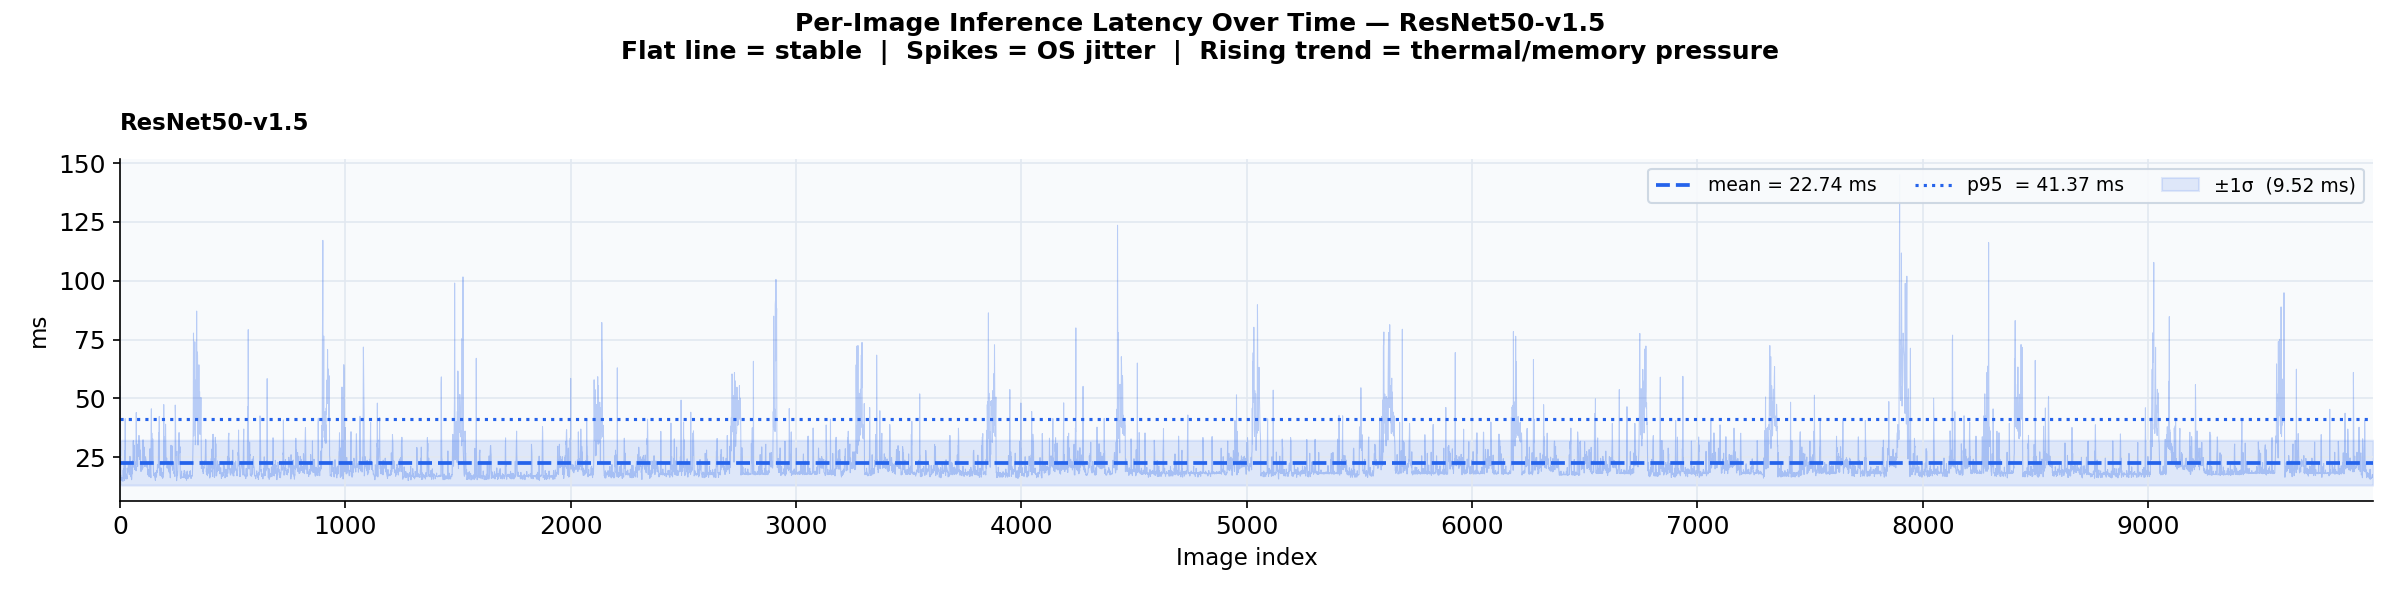
\includegraphics[width=\textwidth]{img/pics updated hiararchy pfe/Per-Model Latency Over Time/1-241-1.png}
    \caption{Latency distribution --- ResNet50-v1.5.}
    \label{fig:m1_hist_resnet50}
\end{figure}

\begin{figure}[p]
    \centering
    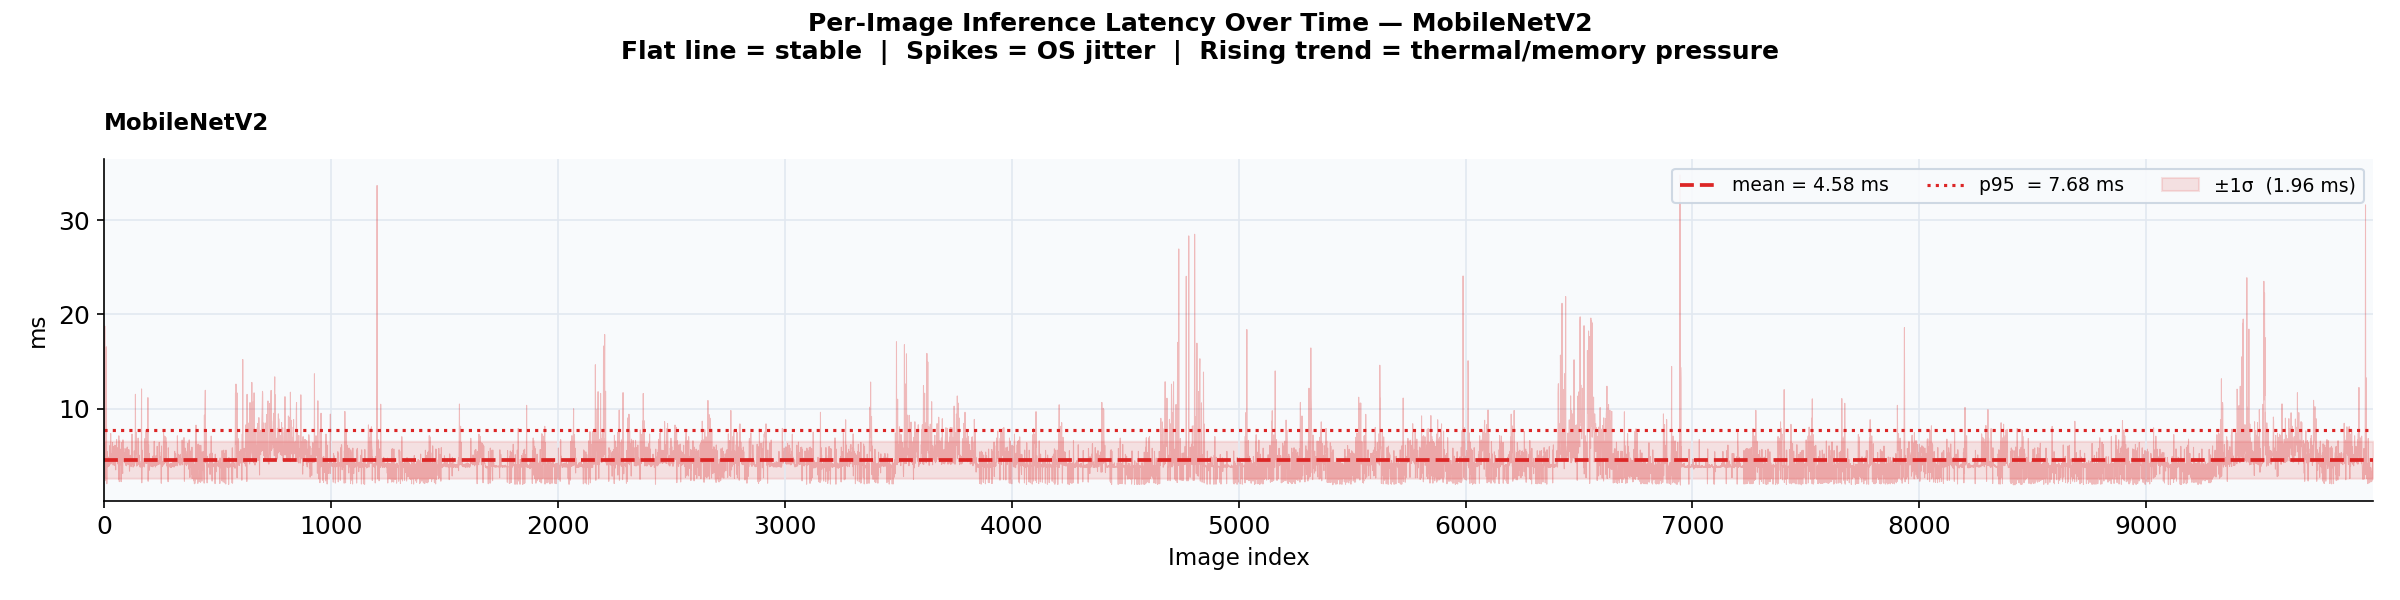
\includegraphics[width=\textwidth]{img/pics updated hiararchy pfe/Per-Model Latency Over Time/1-241-2.png}
    \caption{Latency distribution --- MobileNetV2.}
    \label{fig:m1_hist_mbv2}
\end{figure}

\begin{figure}[p]
    \centering
    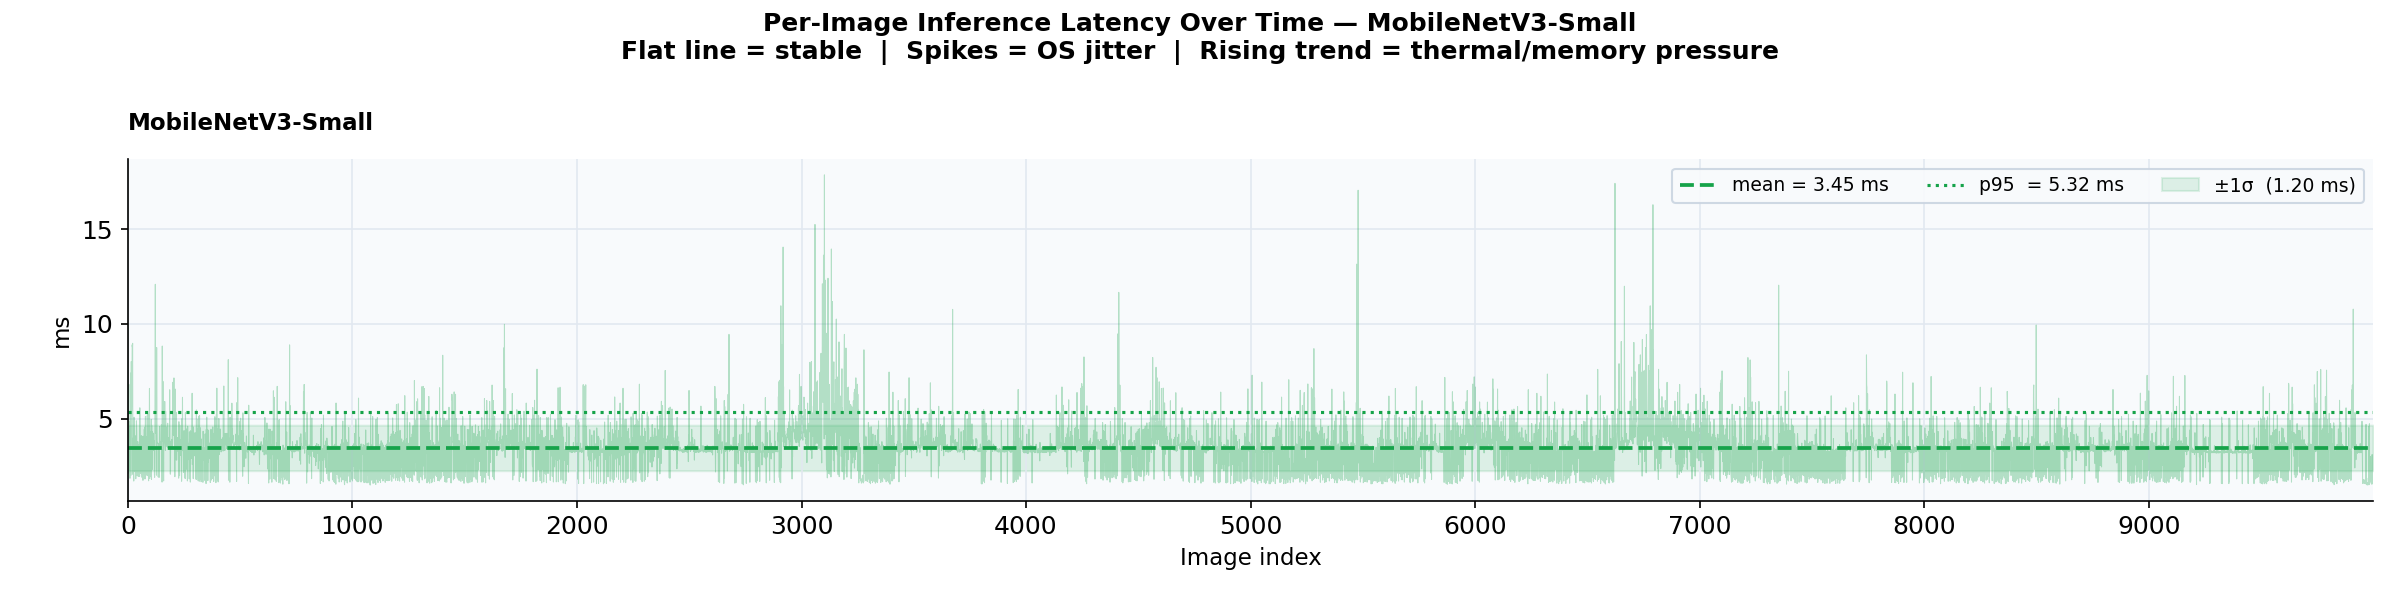
\includegraphics[width=\textwidth]{img/pics updated hiararchy pfe/Per-Model Latency Over Time/1-241-3.png}
    \caption{Latency distribution --- MobileNetV3-Small.}
    \label{fig:m1_hist_mbv3small}
\end{figure}

\begin{figure}[p]
    \centering
    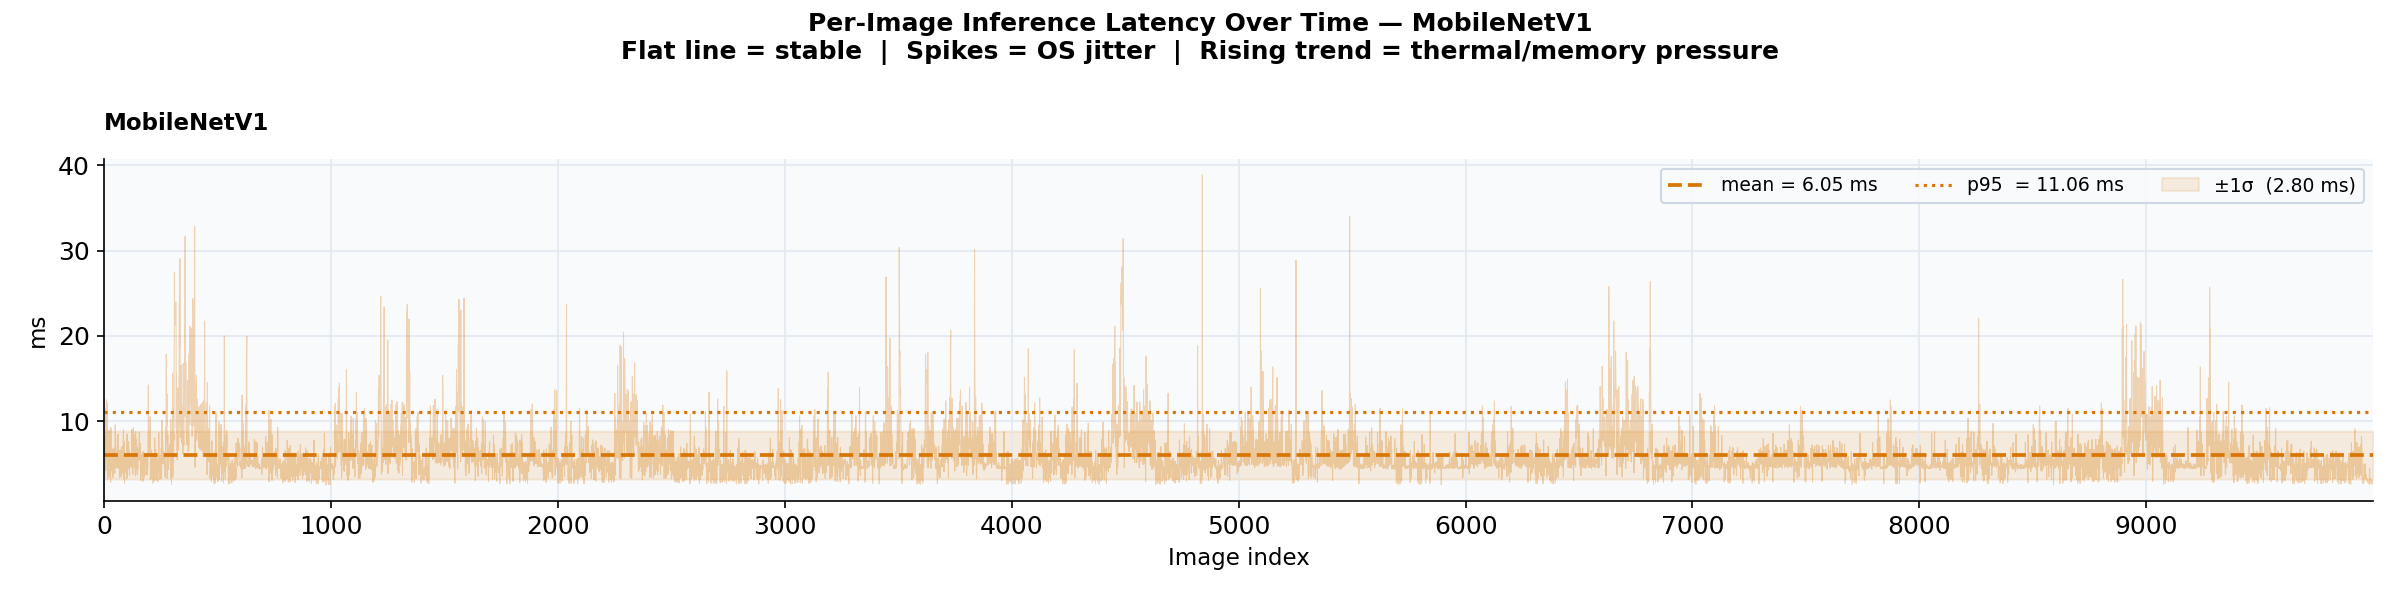
\includegraphics[width=\textwidth]{img/pics updated hiararchy pfe/Per-Model Latency Over Time/1-241-4.png}
    \caption{Latency distribution --- MobileNetV1.}
    \label{fig:m1_hist_mbv1}
\end{figure}

\begin{figure}[p]
    \centering
    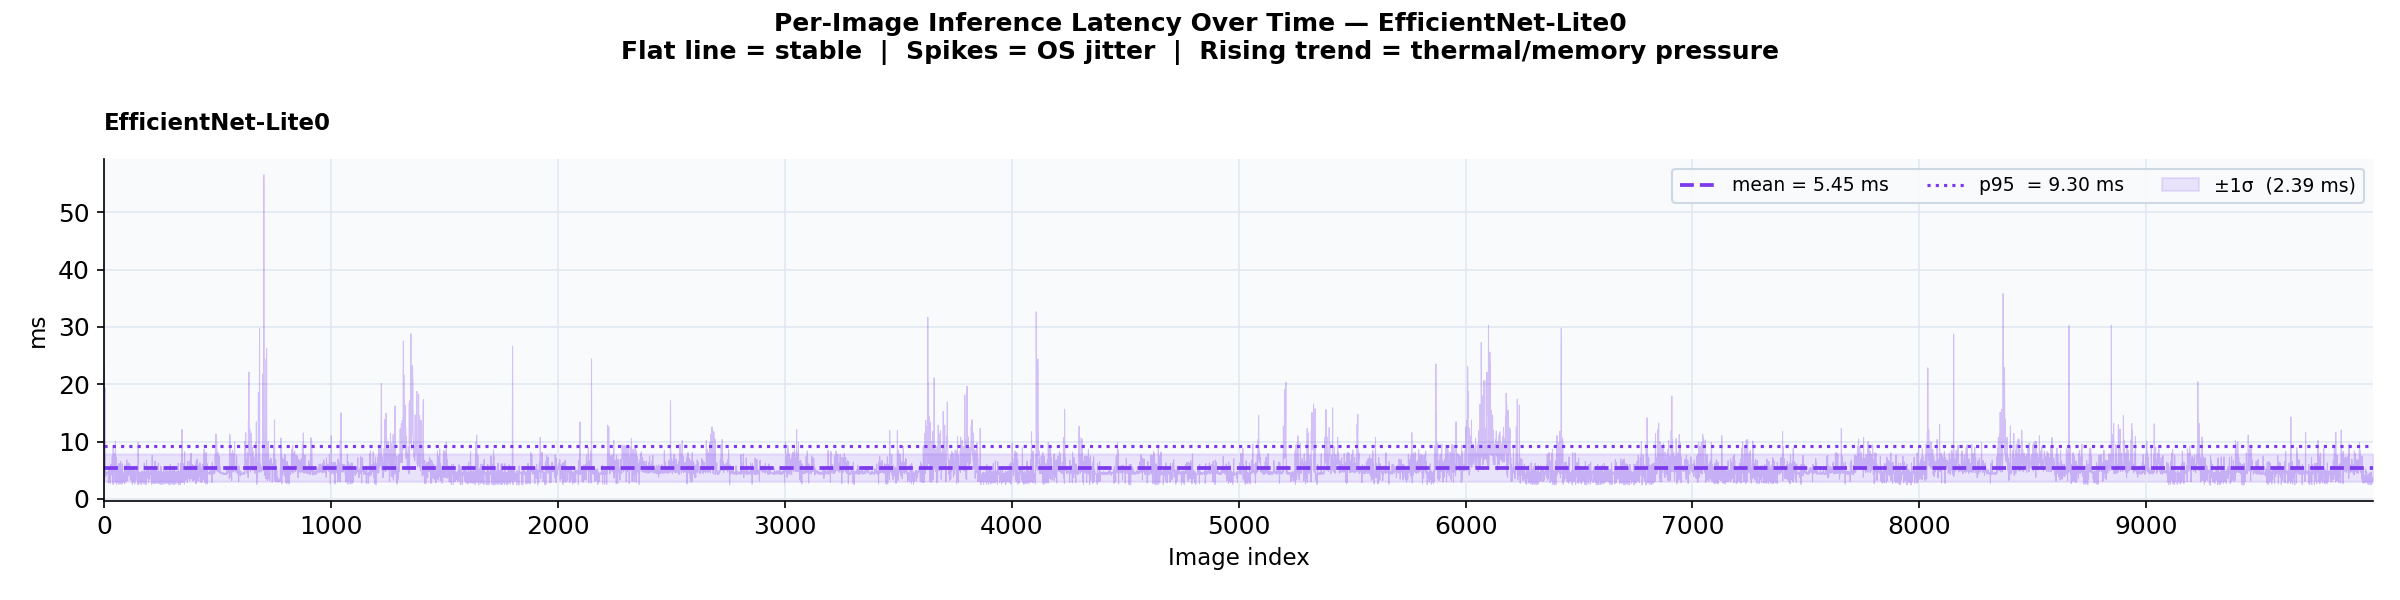
\includegraphics[width=\textwidth]{img/pics updated hiararchy pfe/Per-Model Latency Over Time/1-241-5.png}
    \caption{Latency distribution --- EfficientNet-Lite0.}
    \label{fig:m1_hist_effnet}
\end{figure}

\begin{figure}[p]
    \centering
    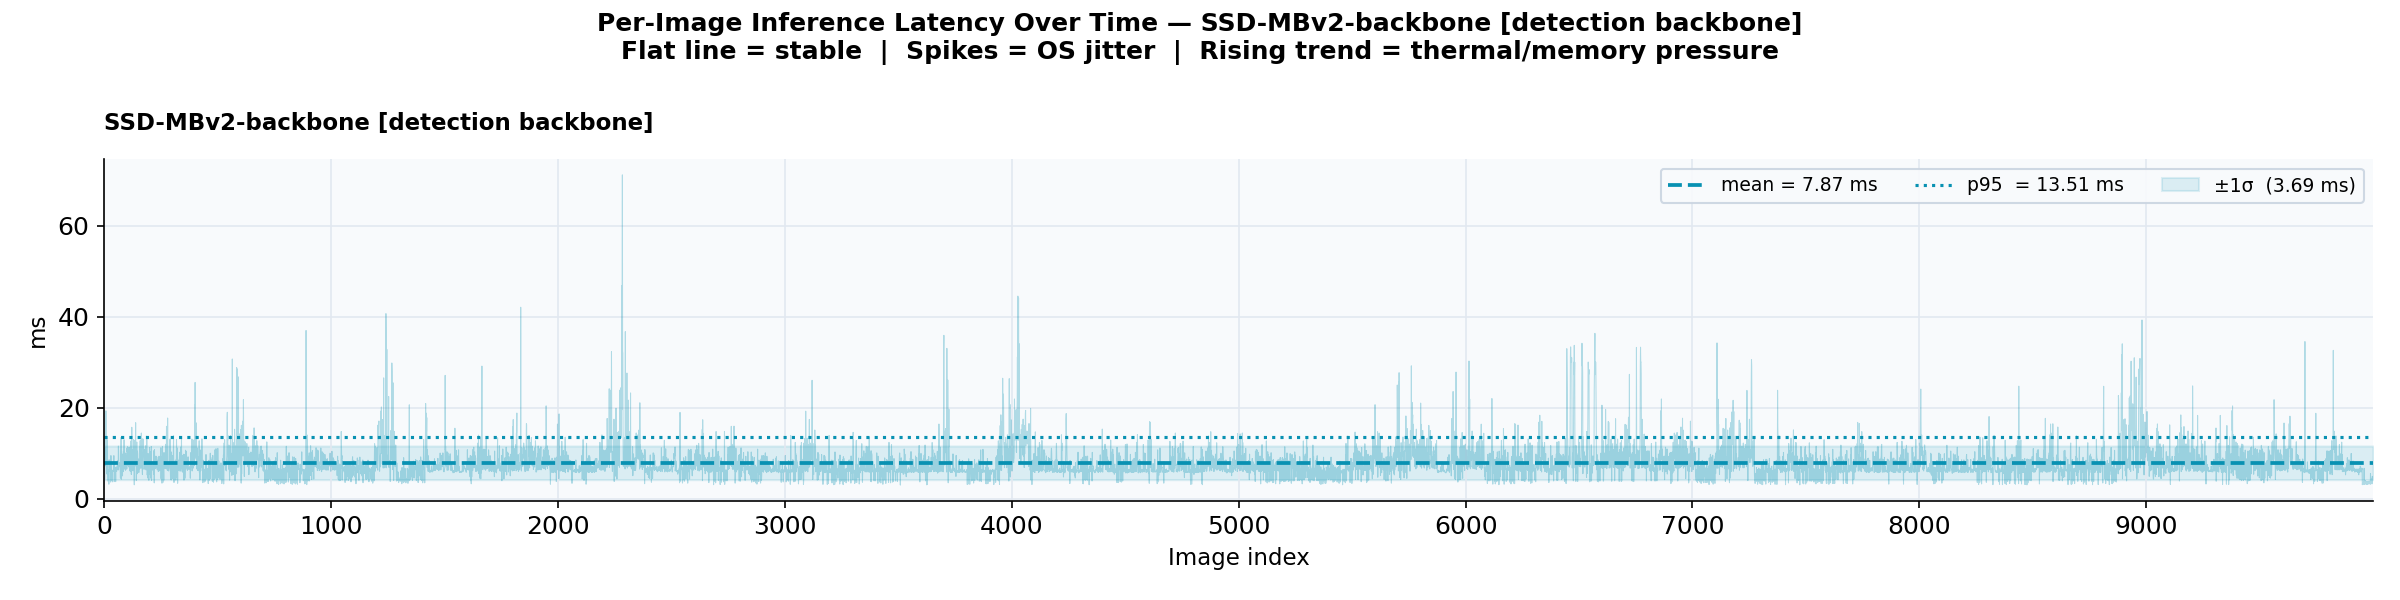
\includegraphics[width=\textwidth]{img/pics updated hiararchy pfe/Per-Model Latency Over Time/1-241-6.png}
    \caption{Latency distribution --- SSD-MBv2-backbone.}
    \label{fig:m1_hist_ssd}
\end{figure}

\clearpage  % flush all remaining floats before continuing

\subsection{Validity Scope and Limitations}

\subsection{Validity Scope and Limitations}

\begin{description}[itemsep=1pt, topsep=3pt]
    \item[\textbf{CPU simulator validity.}] Absolute error versus real
          hardware is expected to be within $\pm15\%$ for mean latency,
          pending physical validation.
    \item[\textbf{NPU simulator validity.}] NPU latency estimates are
          indicative only. They assume perfect INT8 calibration and full
          operator support. Unsupported operators would fall back to CPU,
          increasing real latency.
    \item[\textbf{Accuracy.}] All accuracy numbers derive from real
          \texttt{float32} forward passes. INT8 quantisation effects on
          accuracy must be evaluated on physical hardware with the NXP eIQ
          toolkit.
\end{description}

% =============================================================================
\section{Methodology 3: QEMU User-Mode ARM64 Emulation}
\label{sec:m3_design}
% =============================================================================

\subsection{Overview and Motivation}

Methodology~3 attempts to \emph{actually execute} real ARM64 machine code on
the x86 host using QEMU's user-mode emulation
(\texttt{qemu-aarch64-static}), inside a Docker container running a genuine
ARM64 build of ONNX Runtime. As documented below, QEMU's translation overhead
completely dominates the measured execution time, making this approach
infeasible for inference benchmarking.

\subsection{Two-Stage Docker Image Build}

\begin{enumerate}[itemsep=1pt, topsep=3pt]
    \item \textbf{Stage~A — ARM64 builder:} A genuine \texttt{linux/arm64}
          Ubuntu~22.04 image produces authentic AArch64 ELF binaries:
          Python~3.10, \texttt{numpy}~1.24.4, \texttt{Pillow}~10.4.0, and
          \texttt{onnxruntime}~1.16.3.
    \item \textbf{Stage~B — x86 runner:} Starting from \texttt{amd64}
          Ubuntu~22.04, the ARM64 files are copied into
          \texttt{/opt/arm64\_sysroot/}. The \texttt{qemu-aarch64-static}
          binary is registered with the kernel via \texttt{binfmt\_misc} for
          transparent ARM64 interception.
\end{enumerate}

A wrapper script \texttt{arm64-python} launches the ARM64 Python interpreter
through QEMU with \texttt{OMP\_NUM\_THREADS=4} and
\texttt{ORT\_NUM\_THREADS=4}, mirroring the four-core Cortex-A53 cluster.

\begin{lstlisting}[language=bash,
    caption={The \texttt{arm64-python} wrapper script.}]
#!/bin/bash
exec qemu-aarch64-static \
    -L /opt/arm64_sysroot \
    -E "LD_LIBRARY_PATH=/opt/arm64_sysroot/usr/lib/aarch64-linux-gnu:..." \
    -E OMP_NUM_THREADS=4 \
    -E ORT_NUM_THREADS=4 \
    /opt/arm64_sysroot/usr/bin/python3.10 "$@"
\end{lstlisting}

\subsection{Pipeline Stages}

The orchestrator (\texttt{lrun\_benchmark.py}) runs six stages:
Stage~1 (Docker build), Stage~2 (setup: data download, ONNX export, config),
Stage~2b (ARM64 execution verification via \texttt{platform.machine()}),
Stage~3 (ARM64 inference via \texttt{linference\_qemu\_native.py}),
Stage~4 (statistical metrics), and Stage~5 (visualisation).

\subsection{Observed Failure and Root-Cause Analysis}

Stages~1 and~2 completed normally. Stage~3 correctly printed
\texttt{machine=aarch64} and loaded the ONNX model in $\approx18{,}340$~ms.
The three-run warm-up loop then started and did not return within one hour, at
which point the pipeline was manually terminated.

Three compounding factors explain the extreme slowdown:

\begin{enumerate}[itemsep=1pt, topsep=3pt]
    \item \textbf{Translation overhead:} Every ARM64 instruction block not
          previously seen must be decoded and translated to x86 before
          execution. A single ResNet-50 forward pass involves tens of millions
          of unique instruction sequences on the first call.
    \item \textbf{NEON SIMD emulation:} ONNX Runtime's ARM MLAS kernels use
          ARM NEON (128-bit SIMD) intrinsics. QEMU TCG decomposes each
          128-bit NEON instruction into many scalar x86 operations.
    \item \textbf{No host AVX acceleration:} The ARM64 MLAS kernels are
          compiled for AArch64 only. Even though the host CPU has AVX2, QEMU
          cannot redirect the ARM code to use it.
\end{enumerate}

\begin{table}[H]
\centering
\caption{Summary of Methodology~3 outcomes.}
\label{tab:m3_summary}
\begin{tabular}{ll}
\toprule
\textbf{Attribute} & \textbf{Value / Outcome} \\
\midrule
Emulation mode            & QEMU TCG user-mode (\texttt{qemu-aarch64-static}) \\
Host architecture         & x86\_64 Linux \\
Guest architecture        & AArch64 (ARMv8-A) \\
ORT version               & 1.16.3 (AArch64 native binary) \\
Warm-up runs configured   & 3 \\
Warm-up completion status & Not completed within 1~hour \\
Decision                  & \textbf{Aborted --- approach not viable} \\
\bottomrule
\end{tabular}
\end{table}

\subsection{Lessons Learned}

QEMU TCG is excellent for functional testing and software porting but provides
no timing fidelity relative to real ARM64 silicon. For workloads dominated by
large matrix multiplications inside ONNX Runtime's ARM NEON MLAS kernels, the
gap between QEMU TCG speed and real hardware speed is so large that measured
latencies carry no practical meaning for embedded deployment decisions. The
physics-based simulation of Methodology~2 produces grounded latency estimates
in minutes rather than hours.

% =============================================================================
\section{Architectural Design}
\label{sec:architectural_design}
% =============================================================================

\subsection{Physical Architecture}

The benchmarking environment spans a host x86-64 workstation running the
physics-based simulators (Methodology~2), the ONNX Runtime x86 installation
(Methodology~1), and the Docker engine providing the containerised ARM64
environment (Methodology~3).

% ---- PLACEHOLDER: Physical architecture diagram ----
% A block diagram showing: Host PC -> [M1: ORT x86 | M2: ARMCPUSimulator +
% ARMNPUSimulator | M3: Docker + QEMU] -> Simulated i.MX8M Plus
% \begin{figure}[H]
%     \centering
%     \includegraphics[width=\textwidth]{vis/physical_architecture.png}
%     \caption{Physical architecture of the emulation and simulation
%              environment.}
%     \label{fig:physical_arch}
% \end{figure}

\subsection{Data Flow Architecture}

\begin{enumerate}[itemsep=1pt, topsep=3pt]
    \item ONNX models and Tiny-ImageNet dataset are prepared once and shared
          across all methodologies.
    \item Each methodology executes inference and writes raw latency vectors
          to JSON files.
    \item Metrics scripts compute statistical summaries and write CSV files.
    \item Visualisation scripts generate comparative plots from JSON/CSV.
\end{enumerate}

% =============================================================================
\section{Technology Choices}
\label{sec:technology_choices}
% =============================================================================

\subsection{Why ONNX Runtime}

ONNX Runtime provides cross-platform execution providers
(\texttt{CPUExecutionProvider} for x86 and ARM CPU,
\texttt{VsiNpuExecutionProvider} for Vivante NPU) through a unified API,
enabling direct comparison across hardware targets using the same model files.
Opset~17 covers all selected architectures. ONNX Runtime is the reference
engine for MLPerf~Tiny, ensuring methodology alignment with industry-standard
benchmarks.

\subsection{Why Physics-Based Simulation over Pure QEMU Emulation}

The failure of Methodology~3 empirically validated the physics-based approach:
(1) \textbf{computational feasibility} — full 10\,000-image benchmark in
minutes versus infeasible multi-day QEMU runtime; (2) \textbf{timing fidelity}
— latency estimates grounded in real micro-architectural parameters rather than
emulator overhead; (3) \textbf{configurability} — all parameters exposed in a
single JSON file; (4) \textbf{transparency} — each physical effect is a
separate, documented step.

\subsection{Why the Two-Pass Calibration Strategy}

The 200-image calibration pass resolves the circular dependency between the
ARM CPU and NPU simulators at minimal cost (2\% of the full dataset), providing
a stable estimate of $\bar{L}_{\text{ARM}}^{\text{calib}}$.

\subsection{Simulation Parameter Choices}

Key parameter justifications:
\begin{itemize}[itemsep=1pt, topsep=3pt]
    \item $p_{\text{mem}}=4\%$: midpoint of the 3--5\% contention rate
          reported for i.MX~8 family boards under typical Yocto Linux load.
    \item $f_{\text{mem}}=1.35$: upper end of the 30--40\% stall penalty
          reported in NXP i.MX~8M~Plus application notes.
    \item $\text{CV}_{\text{NPU}}=3\%$: consistent with NXP eIQ benchmark
          reports on the GC7000UltraLite (2--4\% range).
    \item $p_w=15\%$: based on LPDDR4/L2 latency ratio
          ($\sim60$~ns\,/\,$\sim10$~ns) and proportion of memory-bound
          operations in MobileNet-family models.
    \item Thermal onset at image~200: reflects the $\sim30$--60~s
          steady-state warm-up time of embedded SoCs at typical frame rates.
\end{itemize}

% =============================================================================
\section{Comparative Results}
\label{sec:m_results}
% =============================================================================

\subsection{Methodology Comparison}

\begin{table}[H]
\centering
\caption{Summary comparison of the three benchmarking methodologies.}
\label{tab:method_compare}
\resizebox{\textwidth}{!}{%
\begin{tabular}{lccc}
\toprule
\textbf{Attribute} & \textbf{Methodology~1} & \textbf{Methodology~2}
    & \textbf{Methodology~3} \\
\midrule
Execution target  & x86 CPU (real)    & x86 + ARM sim        & AArch64 (QEMU) \\
Latency type      & Measured          & Measured + simulated & Emulated (aborted) \\
ARM accuracy      & N/A               & $\pm15\%$ (estimated)& Would be exact \\
NPU estimate      & None              & Indicative (INT8)    & None \\
Hardware required & x86 workstation   & x86 workstation      & x86 + Docker \\
Completion status & \textbf{Complete} & \textbf{Complete}    & \textbf{Aborted} \\
Runtime           & $\sim$minutes     & $\sim$minutes        & $\sim$hours--days \\
Primary limitation& No ARM estimate   & Analytic model only  & TCG slowdown \\
\bottomrule
\end{tabular}}
\end{table}

\subsection{Key Findings}

\begin{enumerate}[itemsep=1pt, topsep=3pt]
    \item \textbf{MobileNetV1} and \textbf{EfficientNet-Lite0} are the most
          NPU-compatible architectures ($8.33\times$ and $7.14\times$ speedup,
          respectively).
    \item \textbf{MobileNetV3-Small} achieves the lowest x86 latency
          (3.45~ms) but its SE blocks reduce NPU efficiency ($5.00\times$
          speedup vs.\ $8.33\times$ for V1).
    \item \textbf{ResNet50-v1.5} provides the highest accuracy (30.6\%) but
          is the least efficient on both CPU and NPU due to large weight
          tensors exceeding SRAM capacity.
    \item \textbf{Physics-based simulation} produces actionable latency
          estimates in minutes; QEMU instruction-level emulation is
          computationally infeasible for this workload class.
\end{enumerate}

\subsection{Reproducibility}

The pipeline is fully deterministic given \texttt{seed=42} and the canonical
\texttt{pairing\_manifest.csv} ordering. Results are sensitive to CPU
frequency governor, background workload, ONNX Runtime version, and
Pillow/libjpeg version.

% =============================================================================
\section*{Conclusion}
% =============================================================================

This chapter presented a three-methodology emulation and simulation framework
for benchmarking ONNX model inference targeting the NXP i.MX~8M~Plus.
Methodology~1 established that MobileNetV3-Small offers the best x86 latency
(3.45~ms) while the high CV (0.35--0.47) motivated the embedded deployment
study. Methodology~2 delivered a six-effect physics-based simulation producing
ARM CPU and NPU latency estimates in minutes, identifying MobileNetV1
($8.33\times$ NPU speedup) and EfficientNet-Lite0 ($7.14\times$, 31.7\%
accuracy) as the most NPU-compatible architectures. Methodology~3 was
formally attempted and abandoned after the QEMU TCG warm-up phase exceeded
one hour, providing a concrete data point on the infeasibility of
instruction-level emulation for neural network benchmarking.

The next chapter will present the transition to physical hardware validation,
where the simulation estimates from Methodology~2 will be compared against
real measurements on the NXP i.MX~8M~Plus board.